\documentclass[12pt]{article}
\usepackage[utf8]{inputenc}

\usepackage{booktabs}
\usepackage{pdflscape}
\usepackage{graphicx}
\usepackage{hyperref}
\usepackage{setspace}
\usepackage{natbib}
\usepackage[left=1in,right=1in,top=1in,bottom=1in]{geometry}
%\usepackage{titling}


\hypersetup{
    bookmarks=true,         % show bookmarks bar?
    unicode=false,          % non-Latin characters in Acrobat’s bookmarks
    pdftoolbar=true,        % show Acrobat’s toolbar?
    pdfmenubar=true,        % show Acrobat’s menu?
    pdffitwindow=false,     % window fit to page when opened
    pdfstartview={FitH},    % fits the width of the page to the window
    pdftitle={My title},    % title
    pdfauthor={Author},     % author
    pdfsubject={Subject},   % subject of the document
    pdfcreator={Creator},   % creator of the document
    pdfproducer={Producer}, % producer of the document
    pdfkeywords={keyword1} {key2} {key3}, % list of keywords
    pdfnewwindow=true,      % links in new PDF window
    colorlinks=true,       % false: boxed links; true: colored links
    linkcolor=red,          % color of internal links (change box color with linkbordercolor)
    citecolor=black,        % color of links to bibliography
    filecolor=magenta,      % color of file links
    urlcolor=black           % color of external links
}


\title{
The Effect of Forced Coexistence \\ on Native American Health Outcomes \\ 
{\small \sc Economics 381}
}
\author{Kevin Chen \\ Chris Wilkinson}


\begin{document}
%\setlength{\droptitle}{-9em} 

\maketitle

\begin{abstract}
Are Native American health outcomes lower in states and regions in which the US government forcefully integrated historically autonomous sub-tribal bands? This paper explores this question using a differences-in-differences strategy over a spatial dimension. We stratify data on Native American health outcomes by region/state, and then by period. We find that individuals' perceptions of their own health are lower in regions that were subject to forced coexistence. We find that adult mortality per hundred thousand is higher in states whose governments historically forced Native American groups to coexist.
\end{abstract}

\newpage

\doublespacing

% % % % % % % % % % % % % % % %
% % % % % % % % % % % % % % % %
% % % % % % % % % % % % % % % %
% % % % % % % % % % % % % % % %
% % % % % % % % % % % % % % % %
% % % % % % % % % % % % % % % %
% % % % % % % % % % % % % % % %
% % % % % % % % % % % % % % % %
% % % % % % % % % % % % % % % %
% % % % % % % % % % % % % % % %
% 1 page
\section{Introduction}
Are Native American health outcomes lower in states and regions in which the US government forcefully integrated historically autonomous sub-tribal bands?  This paper aims to answer that question in order to examine the broader questions, such as the way conflict or lack of intra-societal cohesion can affect individuals’ health over long periods of time. This is especially important for Native Americans, as they are the only group which has been systematically moved and forced to live with formerly hostile groups.  However, given the variety and complexity of Native American cultures, it is likely that on the whole the effects we find are due to overall effects of social cohesion on health outcomes for most people as opposed to a specific trait about Native Americans.  This would suggest that the question is relevant at a much larger scale, where social strife and conflict could be worsening health outcomes and healthcare delivery across the nation at large.

This paper attempts to answer this question by using a differences-in-differences strategy with spatial and temporal dimensions.  We stratify data on Native American health outcomes by region and state, and then by period based on the CDC’s 1998-2012 database of Native American health outcomes.  The crux of our strategy relies on a forced integration instrumental variable for Native Americans coined by Christian Dippel in his 2010 paper \emph{Forced Coexistence and Economic Development: Evidence from Native American Reservations}.  In the Pacific and some Mountain states, historical mining rushes incentivized the U.S. government to provide less land to the Native Americans in these areas.  Consequently, reservations in these states experienced the forced integration and coexistence with other Native American nations.  By comparing the health outcomes of Native Americans in these states over time, we separate and find the statistical effects of forced coexistence solely on health outcomes.

The overall effects of forced coexistence are somewhat complex, though the overall trend of health outcomes, even having separated out income, is clearly downward for the Native Americans in our forced coexistence regions. 
One of the ways we proxy for health outcomes is by comparing individuals' self-reported health statuses, which are either excellent, good, or fair/poor.
We find that individuals' perceptions of their own health are lower in regions that were subject to forced coexistence. 
However, we find that the lion's share of this difference is caused by a fall in the percentage of people who report \emph{excellent} health and an increase in the share of those who report only \emph{good} health.
That is, whether the region was subject to forced coexistence has little effect on the percentage of people that perceive they are of poor health. 
We theorize that much of this effect may stem from the relative nature of health perception, where individuals measure their health by looking at their neighbors, despite the overall health of the community being lower.

In more concrete results, we find that adult mortality per hundred thousand is higher in states whose governments historically forced Native American groups to coexist, though the actual mechanism for this change is unclear because many of the important causes of death in forced coexistence communities did not feature a statistically significant change when compared to other Native American communities.

The policy implications of these findings are somewhat difficult to pinpoint.  
It would be highly costly to move Native American groups onto new reserves, so we first recommend further research into the diseases and other health conditions which are driving the gap in Native American health. 
We also recommend improving the delivery of healthcare, especially in the public sector within the reservations to try to make it ethnically blind. 
On the larger scale, we recommend further research into health outcomes in the Southern United States, where slavery and desegregation has created similar forced coexistence among formerly unequal or hostile groups.  


% % % % % % % % % % % % % % % %
% % % % % % % % % % % % % % % %
% % % % % % % % % % % % % % % %
% % % % % % % % % % % % % % % %
% % % % % % % % % % % % % % % %
% % % % % % % % % % % % % % % %
% % % % % % % % % % % % % % % %
% % % % % % % % % % % % % % % %
% % % % % % % % % % % % % % % %
% % % % % % % % % % % % % % % %
% 2 pages
\section{Literature}
%motivation, discuss 2-3 key articles, what are their shortcomings, what's left unanswered, external validity problems?
\cite{dippel2010forced} finds that forced integration lowers per capita incomes today by 30 percent. However, he does not look at what effect forced coexistence might have on health.

There are many studies on Native American health outcomes. 
\cite{levin2002geographic} show that the prevalence of cardiovascular disease is higher amongst tribes than in their surrounding states.
\cite{harwell2001cardiovascular} show that cardiovascular disease is more prevalent among American Indians than non-Indians.
\cite{patel2013health} writes about Native Americans perceive their diabetes.
\cite{beals2003racial} compare alcohol use in two reservations to national data.
\cite{may2005outcome} evaluate a public health approach to suicide prevention in a reservation.

There have been a few studies that have explored the effects of political, geopolitical, historical, and economic factors on the prevelance and development of several prominent diseases, such as diabetes (\cite{patchell2014role}), pneumonia, tuberculosis, heart disease, and cancer (\cite{heiner2014demographic}).

There have been studies that explore health disparities.
\cite{mcguire2008new} analyze disparities in mental health and mental healthcare.
\cite{watson2006public} shows how federal sanitation interventions have reduced incidence of disease on Indian reservations and have been responsible for the convergence of Native American and White infant mortality.
\cite{jones2006persistence} details all of the etiologies that exist to try to explain the persistence of American Indian health disparities, and he argues that blaming incidence of disease on genetics is dangerous, as it reduces the obligation to intervene. More likely, disparities exist due to socio-economic inequality.

None of these consider the effect of forced integration on health outcomes.

% % % % % % % % % % % % % % % %
% % % % % % % % % % % % % % % %
% % % % % % % % % % % % % % % %
% % % % % % % % % % % % % % % %
% % % % % % % % % % % % % % % %
% % % % % % % % % % % % % % % %
% % % % % % % % % % % % % % % %
% % % % % % % % % % % % % % % %
% % % % % % % % % % % % % % % %
% % % % % % % % % % % % % % % %
% 1-2 pages
\section{Data}
The data comes from the Center for Disease Control and Prevention (CDC). We use two separate data sets downloaded from the CDC's health interactive database.

\subsection{Adult mortality data}
Table~\ref{sumstat} shows summary statistics about adult mortality per hundred thousand people.

\begin{table}[htbp]\centering \caption{Summary statistics \label{sumstat}}
\begin{tabular}{ | l || c | c | c |}\hline\hline
%\multicolumn{1}{c}{\textbf{Variable}} & \textbf{Mean} & \textbf{Std. Dev.} & \textbf{N}\\ \hline
\textbf{Variable} & \textbf{Mean} & \textbf{Std. Dev.} & \textbf{N} \\\hline
%state &  &   & 0\\
%years & 2.5 & 1.118  & 2080\\
%cause & 5.5 & 2.873  & 2080\\
%mortality & 199.474 & 261.175  & 1304\\
%state\_abbrev &  &   & 0\\
all\_causes & 672.272 & 372.953  & 198\\\hline
cancer & 137.856 & 77.035  & 170\\\hline
diabetes & 58.477 & 30.299  & 90\\\hline
cardio & 208.839 & 109.973  & 184\\\hline
heart\_disease & 160.079 & 83.184  & 172\\\hline
ischemic & 111.496 & 63.119  & 155\\\hline
heart\_attack & 49.452 & 26.794  & 90\\\hline
stroke & 46.482 & 19.866  & 78\\\hline
respiratory & 49.988 & 28.819  & 77\\\hline
cirrhosis & 34.876 & 20.879  & 90\\
%forced\_coex & 0.115 & 0.32  & 2080\\
%\_est\_est1 & 0.095 & 0.294  & 2080\\
%\_est\_est2 & 0.082 & 0.274  & 2080\\
%\_est\_est3 & 0.043 & 0.204  & 2080\\
%\_est\_est4 & 0.083 & 0.275  & 2080\\
%\_est\_est5 & 0.037 & 0.189  & 2080\\
%\_est\_est6 & 0.043 & 0.204  & 2080\\
\hline
\end{tabular}
\end{table}


\subsection{Self-reported health status data}
The first data set contains the self-reported health status for Native Americans, which is measured as excellent, good, or fair/poor, and it is measured in percent as well as base count.  The data takes all of reported data from the Native American population of the U.S. and segments it by region of the country, by income status (poor, near poor, and non-poor) and by year from 1998-2012 in 3 year segments.

Figure~\ref{fig:health_status_by_income} shows the composition of self-reported health statuses across different income groups: \emph{nonpoor}, the highest income group, has the largest fraction of people who reported they had ``excellent'' health.

Figure~\ref{fig:health_status_by_region} shows the composition of self-reported health statuses across different regions: the northeast has the highest fraction of self-reported ``excellent''s.

\begin{figure}[ht!]
\centering
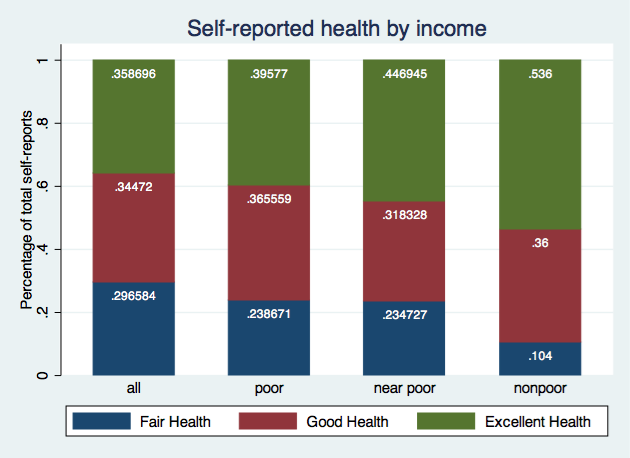
\includegraphics[scale=0.5]{health_status_by_income.png}
\caption{self-reported health by income}
\label{fig:health_status_by_income}
\end{figure}

\begin{figure}[ht!]
\centering
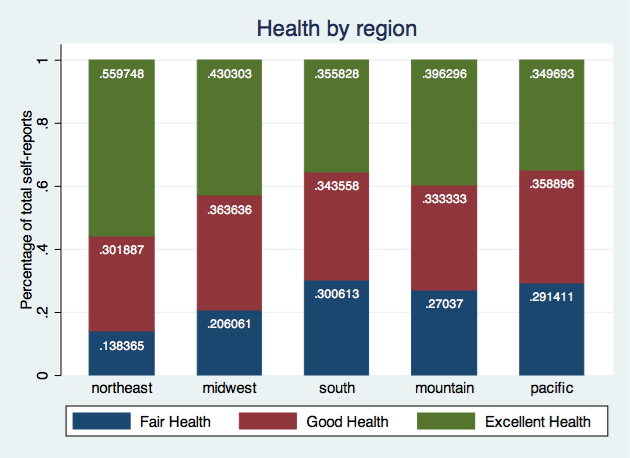
\includegraphics[scale=0.5]{health_status_by_region.png}
\caption{self-reported health by region}
\label{fig:health_status_by_region}
\end{figure}

The second data set contains the cause of death for Native Americans, and it is measured in deaths per 100,000.  The data set is segmented within the U.S. by state and by year 2000-2011 in 3 year segments.  The significant causes of death were cancer, diabetes, major cardiovascular diseases, heart diseases, Ischemic heart disease, heart attack, stroke, respiratory ailments, and liver disease and cirrhosis.

\subsection{Stratification by presence of forced coexistence}
Figure~\ref{fig:reservations} shows states/regions in which autonomous sub-tribal bands experienced forced integration. 

\begin{figure}[ht!]
\centering
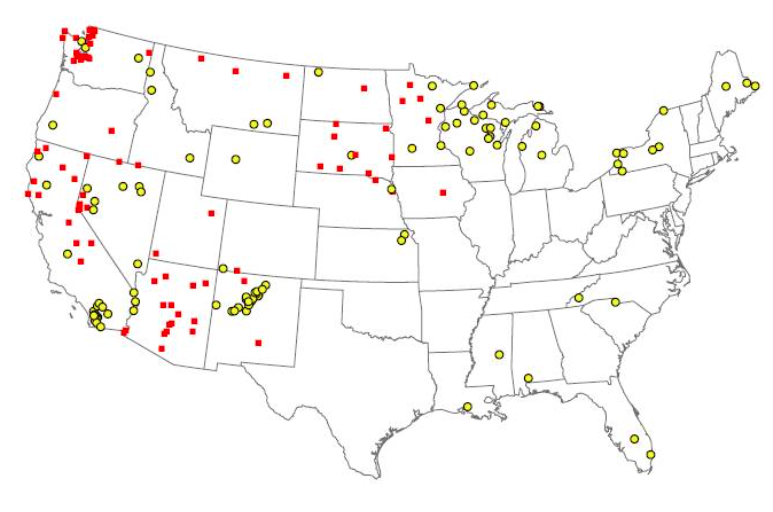
\includegraphics[scale=0.3]{forcedintegration.png}
\caption{Reservations with (red square) and without (yellow circle) forced integration.}
\label{fig:reservations}
\end{figure}

To account for potential selection into forced integration, Dippel uses historical mining rushes (as depicted in Figure~\ref{fig:mining}) as a source of exogenous variation in the government's incentive to forcefully integrate bands onto reservations. 

\begin{figure}[ht!]
\centering
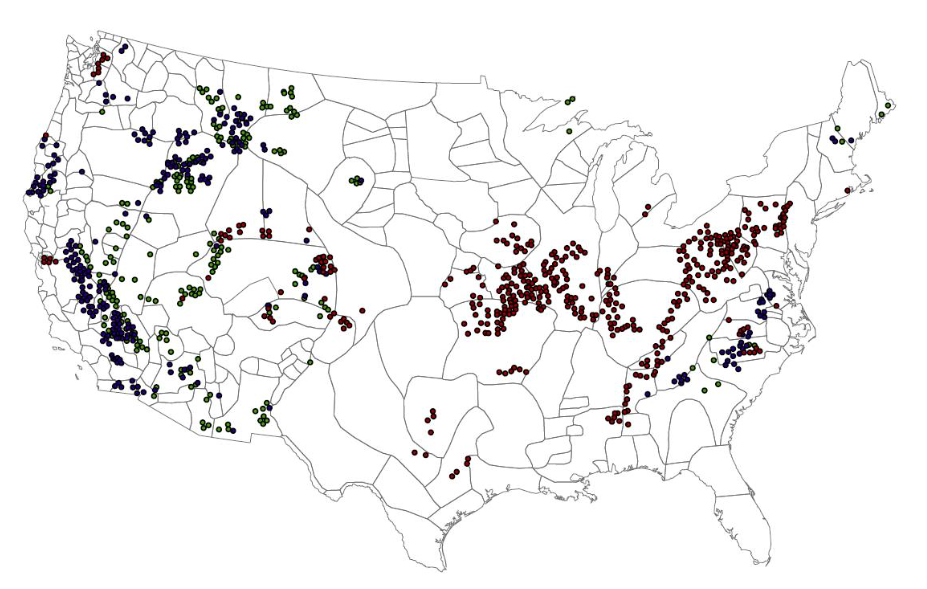
\includegraphics[scale=0.25]{mining.png}
\caption{Geo-database on Mining Clusters in Precious Metals and Coal}
\label{fig:mining}
\end{figure}


% % % % % % % % % % % % % % % %
% % % % % % % % % % % % % % % %
% % % % % % % % % % % % % % % %
% % % % % % % % % % % % % % % %
% % % % % % % % % % % % % % % %
% % % % % % % % % % % % % % % %
% % % % % % % % % % % % % % % %
% % % % % % % % % % % % % % % %
% % % % % % % % % % % % % % % %
% % % % % % % % % % % % % % % %
% 2 pages
% TODO
%\section{Identification Strategy}
%biases of a naive estimate, describe comparison groups, intuition for this comparison


% % % % % % % % % % % % % % % %
% % % % % % % % % % % % % % % %
% % % % % % % % % % % % % % % %
% % % % % % % % % % % % % % % %
% % % % % % % % % % % % % % % %
% % % % % % % % % % % % % % % %
% % % % % % % % % % % % % % % %
% % % % % % % % % % % % % % % %
% % % % % % % % % % % % % % % %
% % % % % % % % % % % % % % % %
\section{Results}

\subsection{Adult mortality}
Table~\ref{adult4} shows that if a state is a forced coexistence state (California, Washington, Montana, Arizona, Idaho, and Utah), then it is expected on average to have higher mortality for ``all causes.'' This reinforces the theory that forced integration has had a detrimental effect on Native American health outcomes. 
Interestingly, however, the forced coexistence variable in Table~\ref{adult4} does not have a statistically significant effect on the individual diseases themselves. 
Tables~\ref{adult2} and \ref{adult3} show similar results.

By contrast, in Table~\ref{adult1} where the only forced coexistence state is California, we find that forced coexistence is less significant on ``all causes'' but has a more significant effect on the indivudal diseases across the board.

\begin{table}[htbp]\centering \caption{Effect of Forced Coexistence (CA) on Adult Mortality\label{adult1}} \begin{tabular}{l*{6}{c}} \toprule
                    &\multicolumn{1}{c}{(1)}&\multicolumn{1}{c}{(2)}&\multicolumn{1}{c}{(3)}&\multicolumn{1}{c}{(4)}&\multicolumn{1}{c}{(5)}&\multicolumn{1}{c}{(6)}\\
                    &\multicolumn{1}{c}{all\_causes}&\multicolumn{1}{c}{cancer}&\multicolumn{1}{c}{diabetes}&\multicolumn{1}{c}{heart\_disease}&\multicolumn{1}{c}{respiratory}&\multicolumn{1}{c}{cirrhosis}\\
\midrule
forced\_coex         &      -269.8&      -57.41&      -39.72&      -55.60&      -26.88&      -20.56\\
                    &     (-1.44)&     (-1.48)&     (-2.65)&     (-1.32)&     (-1.85)&     (-1.96)\\
\addlinespace
Constant            &       677.7&       139.2&       60.24&       161.4&       51.38&       35.79\\
                    &     (25.38)&     (23.36)&     (19.05)&     (25.20)&     (15.47)&     (16.15)\\
\midrule
Observations        &         198&         170&          90&         172&          77&          90\\
\bottomrule
\multicolumn{7}{l}{\footnotesize \textit{t} statistics in parentheses}\\
\end{tabular}
\end{table}

\begin{table}[htbp]\centering \caption{Effect of Forced Coexistence (CA, WA) on Adult Mortality\label{adult2}} \begin{tabular}{l*{6}{c}} \toprule
                    &\multicolumn{1}{c}{(1)}&\multicolumn{1}{c}{(2)}&\multicolumn{1}{c}{(3)}&\multicolumn{1}{c}{(4)}&\multicolumn{1}{c}{(5)}&\multicolumn{1}{c}{(6)}\\
                    &\multicolumn{1}{c}{all\_causes}&\multicolumn{1}{c}{cancer}&\multicolumn{1}{c}{diabetes}&\multicolumn{1}{c}{heart\_disease}&\multicolumn{1}{c}{respiratory}&\multicolumn{1}{c}{cirrhosis}\\
\midrule
forced\_coex         &       8.926&      -9.582&      -26.65&       0.612&      -11.51&      -11.98\\
                    &      (0.07)&     (-0.34)&     (-2.44)&      (0.02)&     (-1.07)&     (-1.56)\\
\addlinespace
Constant            &       671.9&       138.3&       60.85&       160.1&       51.18&       35.94\\
                    &     (24.77)&     (22.79)&     (18.68)&     (24.57)&     (14.77)&     (15.71)\\
\midrule
Observations        &         198&         170&          90&         172&          77&          90\\
\bottomrule
\multicolumn{7}{l}{\footnotesize \textit{t} statistics in parentheses}\\
\end{tabular}
\end{table}

\begin{table}[htbp]\centering \caption{Effect of Forced Coexistence (CA, WA, AZ, UT) on Adult Mortality\label{adult3}} \begin{tabular}{l*{6}{c}} \toprule
                    &\multicolumn{1}{c}{(1)}&\multicolumn{1}{c}{(2)}&\multicolumn{1}{c}{(3)}&\multicolumn{1}{c}{(4)}&\multicolumn{1}{c}{(5)}&\multicolumn{1}{c}{(6)}\\
                    &\multicolumn{1}{c}{all\_causes}&\multicolumn{1}{c}{cancer}&\multicolumn{1}{c}{diabetes}&\multicolumn{1}{c}{heart\_disease}&\multicolumn{1}{c}{respiratory}&\multicolumn{1}{c}{cirrhosis}\\
\midrule
forced\_coex         &       109.1&      -15.61&      -8.462&      -4.298&      -21.08&      -3.883\\
                    &      (1.12)&     (-0.77)&     (-1.01)&     (-0.20)&     (-2.40)&     (-0.66)\\
\addlinespace
Constant            &       663.5&       139.3&       59.98&       160.5&       53.27&       35.52\\
                    &     (24.01)&     (22.42)&     (17.03)&     (24.03)&     (15.36)&     (14.69)\\
\midrule
Observations        &         198&         170&          90&         172&          77&          90\\
\bottomrule
\multicolumn{7}{l}{\footnotesize \textit{t} statistics in parentheses}\\
\end{tabular}
\end{table}

\begin{table}[htbp]\centering \caption{Effect of Forced Coexistence (CA, WA, MT, AZ, ID, UT) on Adult Mortality\label{adult4}} \begin{tabular}{l*{6}{c}} \toprule
                    &\multicolumn{1}{c}{(1)}&\multicolumn{1}{c}{(2)}&\multicolumn{1}{c}{(3)}&\multicolumn{1}{c}{(4)}&\multicolumn{1}{c}{(5)}&\multicolumn{1}{c}{(6)}\\
                    &\multicolumn{1}{c}{all\_causes}&\multicolumn{1}{c}{cancer}&\multicolumn{1}{c}{diabetes}&\multicolumn{1}{c}{heart\_disease}&\multicolumn{1}{c}{respiratory}&\multicolumn{1}{c}{cirrhosis}\\
\midrule
forced\_coex         &       230.2&       12.92&       2.276&       17.14&      -8.214&       5.815\\
                    &      (2.89)&      (0.76)&      (0.31)&      (0.94)&     (-1.01)&      (1.15)\\
\addlinespace
Constant            &       644.4&       136.0&       57.87&       157.7&       51.70&       33.39\\
                    &     (23.21)&     (21.31)&     (15.44)&     (23.05)&     (14.01)&     (13.11)\\
\midrule
Observations        &         198&         170&          90&         172&          77&          90\\
\bottomrule
\multicolumn{7}{l}{\footnotesize \textit{t} statistics in parentheses}\\
\end{tabular}
\end{table}











\subsection{Health status}
Originally there were three income levels: poor, nearpoor, and non-poor. However, to simplify things and work with a convenient binary, we combined poor and nearpoor.

Thus, Table~\ref{ppoor} shows the effect of being poor (or nearpoor) on self-reported health statuses in the Pacific region. Table~\ref{pmpoor} is the same but for the Pacific and Mountain regions.

Using both the Pacific and Mountain regions, we find that for all income groups, living in the regions which featured forced coexistence saw significantly lower levels of excellent health outcomes reported as well as an increased percentage stating their health to be merely good or fair among Native Americans.  Among the poor, who are especially populous among Native Americans, the interaction term between forced coexistence and being poor is statistically significant for percentage reporting good health, and it increases the percentage reporting good by 3.95 percentage points whereas income itself is statistically insignificant.  This suggests that forced coexistence plays a strong role in dropping self-reported health from excellent to good.

However, the interaction terms tell a slightly different story about the cause of these outcomes in potentially dropping health perception from good down to fair.  In tables 2, 3, and 4 the interaction term on forced coexistence and wealth is not statistically significant with regards to fair self-reported health.  This suggests that much of the differences seen in the forced coexistence term on percent of Native Americans reporting fair health are coming from differences in income or in other unexplained variables.  

In the Pacific, where the more speedy and haphazard forced integration occurred due to larger mining rushes, we see somewhat clearer negative results from forced coexistence.  We see the same general results from region and income variables in worsening Native American health, but the interaction terms between forced coexistence and income are more significantly negative.  Among the poor, the interaction variable between forced coexistence and poor income is statistically significantly dropping the percentage reporting excellent health by 3.912 percentage points and at the same time significantly increasing the percentage of people reporting good health by 5.145 percentage points.  This is an even stronger effect than was seen in the combined Pacific and Mountain regions because most of the loss of excellent outcomes among the poor in the combined regions was due to income alone, not due to the combination of income and forced coexistence.

Again though, there is no statistically significant effect of the forced coexistence interaction term on any income group upon the fair outcomes, suggesting that forced coexistence is not drastically worsening poor Native Americans’ health, but rather making it slightly worse, at least in their own perception. 

% % % % % %
\begin{table}[htbp]\centering \caption{Effect of Poor Income on Health Statuses in the Pacific and Mountain Regions\label{pmpoor}} \begin{tabular}{l*{3}{c}} \toprule
                    &\multicolumn{1}{c}{(1)}&\multicolumn{1}{c}{(2)}&\multicolumn{1}{c}{(3)}\\
                    &\multicolumn{1}{c}{percent\_excellent}&\multicolumn{1}{c}{percent\_good}&\multicolumn{1}{c}{percent\_fair}\\
\midrule
forced\_coex         &      -8.632&       4.228&       3.281\\
                    &     (-6.47)&      (4.52)&      (2.18)\\
\addlinespace
income\_poor         &      -5.710&       2.829&       6.709\\
                    &     (-4.86)&      (3.15)&      (4.18)\\
\addlinespace
forced\_poor         &       1.369&       2.591&      -3.513\\
                    &      (0.73)&      (1.91)&     (-1.53)\\
\addlinespace
Constant            &       56.27&       30.15&       18.92\\
                    &     (73.89)&     (54.06)&     (19.32)\\
\midrule
Observations        &         568&         487&         356\\
\bottomrule
\multicolumn{4}{l}{\footnotesize \textit{t} statistics in parentheses}\\
\end{tabular}
\end{table}

\begin{table}[htbp]\centering \caption{Effect of Poor Income on Health Statuses in the Pacific Region\label{ppoor}} \begin{tabular}{l*{3}{c}} \toprule
                    &\multicolumn{1}{c}{(1)}&\multicolumn{1}{c}{(2)}&\multicolumn{1}{c}{(3)}\\
                    &\multicolumn{1}{c}{percent\_excellent}&\multicolumn{1}{c}{percent\_good}&\multicolumn{1}{c}{percent\_fair}\\
\midrule
region\_p            &      -7.662&       5.835&      -2.621\\
                    &     (-6.08)&      (6.80)&     (-1.84)\\
\addlinespace
income\_poor         &      -4.237&       2.461&       4.722\\
                    &     (-3.79)&      (2.96)&      (3.12)\\
\addlinespace
forced\_poor         &      -3.432&       3.433&       1.303\\
                    &     (-2.34)&      (3.17)&      (0.68)\\
\addlinespace
Constant            &       54.79&       30.51&       20.91\\
                    &     (82.36)&     (65.29)&     (25.65)\\
\midrule
Observations        &         568&         487&         356\\
\bottomrule
\multicolumn{4}{l}{\footnotesize \textit{t} statistics in parentheses}\\
\end{tabular}
\end{table}


% % % % % % % % % % % % % % % %
% % % % % % % % % % % % % % % %
% % % % % % % % % % % % % % % %
% % % % % % % % % % % % % % % %
% % % % % % % % % % % % % % % %
% % % % % % % % % % % % % % % %
% % % % % % % % % % % % % % % %
% % % % % % % % % % % % % % % %
% % % % % % % % % % % % % % % %
% % % % % % % % % % % % % % % %
\section{Measurement issues}

% % % % % % % % % % % % % % % %
% % % % % % % % % % % % % % % %
% % % % % % % % % % % % % % % %
% % % % % % % % % % % % % % % %
% % % % % % % % % % % % % % % %
% % % % % % % % % % % % % % % %
% % % % % % % % % % % % % % % %
% % % % % % % % % % % % % % % %
% % % % % % % % % % % % % % % %
% % % % % % % % % % % % % % % %
\section{Discussion}
\subsection{Self-reported health statuses}
\subsubsection{Interpreting the interaction term}

Interestingly, in Table~\ref{pnearpoor}, neither income nor the interaction term has a statistically significant effect on the reported health status of the near poor in the Pacific, suggesting that other variables unique to the region may be playing a large part in the large drop from excellent to good health perception.  Moreover, if these variables were related to income or forced coexistence, they could be clouding our findings.

%The interaction term is an offsetting effect because the two variables are somewhat correlated. In other words, people in forced coexistence areas are also more likely to be poor. Meaning that if we were to only regress \% fair on poor, you would be in part capturing the correlation between being poor and in part being in forced coexistence. So being poor undermines health, being in forced coexistence undermines health. However, being poor in a forced coexistence area is less correlated with the likelihood you think you are in poor health. One possible interpretation is that in forced coexistence communities the poor are comparing their health to others similar to them whereas in the poor in non-forced coexistence communities live in wealthier areas and subjectly evaluate the health to be poorer. It would be interesting to see if you still get this negative interaction effect when looking at the mortality figures as that might help you to distinguish between perceptions vs actual health discrepancies between poor in forced coexistence and non-forced coexistence areas. 

\subsection{Adult mortality}
\subsubsection{The whole, but not the pieces}
Our forced coexistence dummy variable significantly explains on ``all causes'' but has no significance in explaining each individual cause (e.g., cancer, heart attack, stroke). This may be because there is insufficient statistical power to detect differences when split by the different diseases due to small changes (even if equivalent in percentage terms) whereas when they are aggregated there is not this problem. 
% TODO
% Are the coefficients consistent with the aggregate results? Also do the coefficients on the diseases add up to approximately the coefficient you  observe for all diseases?

% % % % % % % % % % % % % % % %
% % % % % % % % % % % % % % % %
% % % % % % % % % % % % % % % %
% % % % % % % % % % % % % % % %
% % % % % % % % % % % % % % % %
% % % % % % % % % % % % % % % %
% % % % % % % % % % % % % % % %
% % % % % % % % % % % % % % % %
% % % % % % % % % % % % % % % %
% % % % % % % % % % % % % % % %
\section{Conclusion}
To conclude, our main findings are that forced coexistence does have a significant effect on individuals’ health outcomes, though not in the way that we imagined.  Rather than decreasing perceptions of health across the board our findings reveal that most of the damage is done in reducing excellent health to more mediocre results.  Moreover, we imagined that in terms of specific diseases, forced coexistence would have more of an effect in certain diseases, perhaps in ones with high contagiousness where social control would have to be exerted to keep the damages down.  Instead, forced coexistence seemed to affect overall health conditions, like mortality, but did not have a statistically significant effect on any one cause of death.

This findings are important because they answer affirmatively that forced coexistence does effect health and because give us some valuable insight on how forced coexistence has damaged the Native American communities. The broad effects of forced coexistence suggest that health is being affected through overall less efficient administration of the reservation as compared to single nation Native American reservations.  This could occur through mechanisms like lower overall income, worse delivery of public medical services, and uncertain reservation medical policies as Native American groups struggle politically. Also, though overall healthiness is damaged, it seems that it is fairly equitable among individuals in a society with forced coexistence, given that no diseases were more prominent and that Native Americans’ perceptions of health were clumped heavily around good.  They were in good health relative to their neighbors though they we’re likely lower than Native Americans in other reservations or off the reservation.  

Of course, further research is required in individual Native American reservations to pinpoint the true causes of these worse health outcomes.  However, given what we now know, we recommend that policies be enacted to increase efficiency of health care delivery within the reservations of the Pacific and Mountain regions which experience forced coexistence.  The exact nature of these programs will depend on the flaws discovered by more pinpointed research, but we expect there to be problems of insufficient information regarding diseases and distant or poorly stocked supply of medical services.  These should be solved by providing subsidies for information and further provision of medicine in a cost effective manner.  In addition to the policy implications, we believe this paper contributes to the literature on the long lasting health consequences of social strife and heavy handed government relocation of ethnic or racial groups.


\newpage
\bibliographystyle{te}
\bibliography{main}


\end{document}
